

\chapter{Methodology}
This chapter presents the solution approach.
Section 4.1 motivates our problem. 
Section 4.2 gives and introduction to supervised learning and presents the algorithms considered in the comparison in detail.
Section 4.3 presents feature selection techniques applied in the computational study. 
Section 4.4 defines the process by which we evaluate the models in order to assess their quality.

\section{Motivation}
From the literature review it has already become apparent that supervised learning is a common way to go. 

\section{Algorithms}

This section shortly introduces the statistical framework of supervised learning \citep{SLFoundations} and then proceeds with the detailed examination of how each approach and algorithm included in our comparison, namely linear models, tree-based ensembles and neural networks, function \citep{friedman2001elements}.

As inputs, supervised learning algorithms receive \textbf{training data} in form of a finite set $ S = \{({x}_{2}, y_2), ({x}_{2}, y_2), \dots, ({x}_{n}, y_n)\}$ of N pairs from $ \mathcal{X} \times \mathcal{Y} $ where $ x_i $ is a \textbf{sample} described by $ p $ features, and is associated to it's corresponding \textbf{label} $ y_i $.
They return a \textbf{hypothesis} $ h: \mathcal{X} \to \mathcal{Y} $ that aims to predict the corresponding label $ y \in Y $ for any $ x \in X $, but especially for unseen samples or i.e. \textbf{test data} $ x \notin S $.
We further assume a joint probability distribution $ P $ over $ \mathcal{X} $ and $ \mathcal{Y} $ each pair is identically and independently distributed according to. 
This assumption allows us to take uncertainties of predictions in form of noise in the training data into account. 
Thus, $ h(x) $ can be treated as a random variable being conditionally distributed with $ P(y | x) $ for a given $ x $, and not as a deterministic function of $ x $.
The prediction accuracy of $ h $ is measured with a  \textbf{loss function} $ L : Y \times Y \to \mathbb{R}^{\geq 0}$.
For a given pair $ ({x}_i, y_i) $, the loss function $ L(y_i, \hat{y}_i) $ represents how far a prediction $ \hat{y_i} $ for the i-th sample $ x_i $ is away from the actual corresponding label $ y_i $. 
The average loss across all $ (x,y) \in S $ is called \textbf{empirical risk}.
Thus, the goal of a supervised learning algorithm is to find the optimal hypothesis $ h^* $ for which the overall empirical risk is minimal: 
\begin{equation}
	h^* = \argmin_{h \in H} \dfrac{1}{n} \sum_{i=1}^{n} L(h(x_i), y_i).
\end{equation}

Predictions can generally be made for either \textbf{regression} or \textbf{classification} problems which differ in the nature of their target variable. 
While regression is used to predict continuous targets $ Y = \mathbb{R} $, classification predicts discrete $ Y $. The arrival time estimation problem is a regression task since we are estimating (continuous) arrival times.
Although various supervised learning models use different mathematical procedures to predict targets, all of them follow the principle of induction, meaning that general rules are inductively inferred from training data. This is also called \textbf{generalization}.  
In order for a model to generalize well, two phenomena have to be avoided: \textbf{Underfitting} and \textbf{Overfitting}. 
Poor predictions on both the training and test data indicate that a model is underfitted, whereas an overfitted model is characterized by very good prediction accuracy for samples $ x \in S $, but poor accuracy on test data.
In supervised learning, this is known as the \textbf{bias-variance tradeoff}. 
A overfitted model is low in bias and high in variance, whereas the same goes vice versa for underfitted models. This dilemma is known as the \textbf{bias-variance tradeoff}. Models high in bias and low in variance are rather simple, e.g. linear regression models. Due to models low in bias and high in variance being able to capture rather complex patterns, they tend to also learn the noise in the training data. 
The key challenge therefore lies in finding a model balancing this tradeoff well and thus having good prediction quality especially on test data. 

For that reason, we consider diverse models covering the wide spectrum of model complexities.
 
\subsection{Linear Models}

Linear regression models assume that every $ y $ can be predicted with a linear combination of the inputs. 
Let $ \textbf{X}^{T} = (X_1, X_2, \dots, X_p) $ denote the input matrix containing $ p $ column vectors with N components each, and $ \hat{Y} = (y_1, y_2, \dots, y_n)$ the column vector with the corresponding real-valued outputs. A linear regression model is a linear combination of parameters $ w $ and column vectors $ X $:
\begin{equation}
h(X) = w_0 + \sum_{j=1}^{p} X_jw_j.
\end{equation}

Parameter $ w_0 $ represents the intercept. A linear model assumes linearity in its parameters, whereas feature vectors $ X \in \textbf{X}^{T} $ can be of any form and arbitrarily transformed. 

In case of a 1- or 2-dimensional feature space, we can visualize the regression model graphically as a straight line or hyperplane respectively in cartesian coordinate systems
One popular way of approximating hypotheses in linear regression is \textit{least squares}, which seeks to find coefficients $ w^{*}_j $, $ j = 1, \dots, p $ that minimize the residual sum of squares across all N pairs the training set $ S $:
\begin{equation}
\argmin_{w} \sum_{i=1}^{N}(y_i - w_0 - \sum_{j=1}^{p} x_{ij}w_j)^2 
\end{equation}

\subsection{Tree-based ensembles}

As shown in the literature review, tree-based ensembles like GBDTs and Random Forests are popular in the field of arrival time estimation. Ensemble learning is motivated by the idea that so called \textit{base learners} (synonym to \textit{model} or \textit{hypothesis}) produce rather inaccurate results on their own, but form an accurate prediction model when they are combined. For tree-based ensembles, decision trees are used as base learners. 
Generally speaking, decision trees partition the feature space into distinct regions and then, in the case of regression, fit a real-valued prediction to each region. 
A single decision tree is given by
\begin{equation}
h(x) = \sum_{m=1}^{M} c_m I(x \in R_m)
\end{equation}
where $ c_m $ is the constant representing the prediction for all samples belonging to the m-th terminal region $ R_m $. Adopting the mean squared error as the loss metric, the predicted constant $ \hat{c}_m $ for each terminal region $ R_m $ is the average of all $ y $ for each $ x \in R_m $:
\begin{equation}
	\hat{c}_m =  \dfrac{1}{N_{R_m}}\sum_{x_i \in R_m}^{} y_i
\end{equation}
with $ N_{Rm} $ being the number of samples in terminal region $ R_m $. Given this, the decision tree algorithm needs to find optimal binary splits. Solving this analytically is computationally infeasible. Therefore, decision trees are constructed in a greedy fashion.
Let $ j $ be the split variable, representing the feature based on which the split of the feature space is done on, and $ s $ its associated split threshold.
The initial partition creates two disjoint regions
\begin{equation}
	R_1 (j,s) = \{X | X_j < s \}, R_{2} = \{X | X_j > s\}.
\end{equation}
The algorithm seeks optimal $ j $ and $ s $ by finding constants that minimize the overall loss, which in our case is measured with the mean squared error, for both terminal regions $ R_1 $ and $ R_2 $:
\begin{equation}\label{minjs}
	\min_{j,s} \bigg [\min_{\hat{c}_1} \sum_{x_i \in R_1(j,s)} \dfrac{1}{2}(y_i - \hat{c}_{2})^2 + \min_{\hat{c}_2} \sum_{x_i \in R_{2}(j,s)} \dfrac{1}{2}(y_i - \hat{c}_{2})^2\bigg]
\end{equation}
Having found the optimal split variable and split threshold, this procedure is repeated for each terminal region until a termination condition holds, e.g. a fixed maximal depth for the tree or a lower bound wrt. number of samples in each terminal region.
\newline
TODO: Disadvantages of decision trees (e.g. prone to overfitting, not as accurate as ensembles)
\newline
\newline
Knowing how CART builds regression trees, we now can advance to tree-based ensemble learning techniques which combine several regression trees to make predictions each in their own way.
The two ensemble learning approaches relevant for this work are \textbf{bagging}, , shorthand for \textit{bootstrap aggregating}, and \textbf{boosting}. 
Algorithms belonging to bagging first create bootstrap data sets $ S^{*} $ by randomly drawing samples with replacement from training data S, fit each $ S^{*b} $ a hypothesis $ h^{*b}(x) $ and take the average across all hypotheses as the bagging estimate: 
\begin{equation}\label{average}
	h_{bag}(x) = \dfrac{1}{B} \sum_{b=1}^{B} h^{*b}(x).
\end{equation}
Since decision trees are low in bias and high in variance due to their ability to capture complex mappings, averaging across all hypotheses reduces the variance because of the strong law of large numbers [<-- TODO: More detailed explanation].
Random Forests belong to the class of bagging algorithms and work as follows:
For an arbitrarily chosen and fixed amount of estimators $ B \in \mathbb{N}$, we create bootstrap data sets $ S^{*b} $ with $ b = 1, \dots, B $ of size $ N $ from the training data $ S $. The b-th regression tree $ T_b $ is grown to $ S^{*b} $ by first selecting a subset of $ m $ features with $ m \leq p $, and then growing a regression tree according to CART as described above.
Having grown each bootstrap data set $ S^{*b} $ its own regression tree $ T_b $, random forest for regression averages across all hypotheses of each regression tree by applying equation \ref{average} and returns
\begin{equation}
h^{B}_{rf}(x) = \dfrac{1}{B} \sum_{b=1}^{B} T_b(x)
\end{equation}
as the bagging estimate.
\newline
\newline
TODO: Introduce concept of boosting and GBDTs before diving deep into technical details.
\newline
\newline
The first step in GBDT is to initialize a model with a constant $ \hat{c} $ that minimizes the overall loss across all training samples.
\begin{equation}
h_{0}(x) =  \argmin_{\hat{c}} \sum_{i=1}^n L(y_i,\hat{c}) \label{gbdt_step1}
\end{equation}
Using mean squared error as the loss metric, the predictor minimizing the overall loss is simply the average of all $ y $.
Given the initial model $ h_0(x) $, M regression trees can now be build sequentially as shown in the following. 
The first step computes pseudo-residuals $ r_{im} $ between the prediction value of the former learner for the i-th sample $ h_{m-1}(x) $ and the actual i-th target for the m-th tree $ y_i $ by deriving the loss function w.r.t to $ h_{m-1}(x) $: 
\begin{equation}
	r_{im}\ = - \bigg[\dfrac{\delta L(y_i, h(x_i))}{\delta h(x_i)}\bigg]_{h(x) = h_{m-1}(x)}
\end{equation} 
for every i-th example.
In the second step, the algorithm fits a regression tree to every $ r_{im} $ and creates disjoint regions $ R_{jm} $ for $j = 1, ..., J_m$. 
In the third step, we compute: 
\begin{equation}
	\hat{c}_{jm} = \argmin_{\hat{c}} \sum_{x_i \in R_{ij}} L(y_i, h_{m-1}(x_i) + \hat{c})
\end{equation}
for every terminal region j in the m-th tree. 
Given this, we now update the former weak learner with the new one:
\begin{equation}
	h_m(x) = h_{m-1}(x) + \alpha \sum_{j=1}^{J_m} \hat{c}_{m}I(x \in R_{jm})
\end{equation}
where $ \alpha $ is the learning rate, and $ I(\cdot) $ is the indicator function.
\newline
\newline
TODO: Explain shortcomings of traditional GBDT and explain why lightgbm implementation is used (e.g. leaf-wise tree growth) (maybe in detail?)

\subsection{Neural Networks for regression}


\begin{figure}[h]
	\centering
	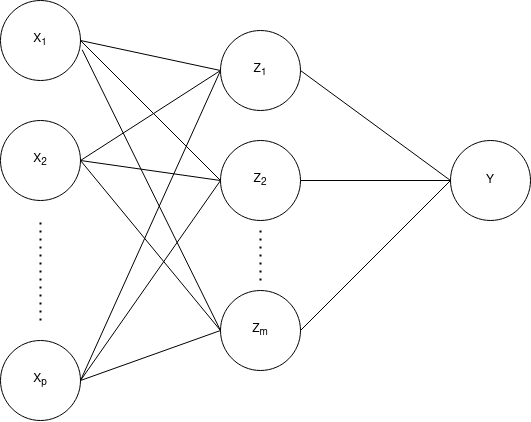
\includegraphics[width=0.5\linewidth]{../simplenn.png}
	\caption{Our neural network architecture to estimate arrival times: a single layer perceptron.}
	\label{fig:nnarchitecture}
\end{figure}


\section{Feature Selection}

As shown, researchers use different feature selection methods. A majority of the presented papers crafts features manually relying on domain expertise, whereas others (e.g \cite{Siripanpornchana2016_AnnWithDbnFS} and \cite{Huang2018_GBDT}) used representation learning techniques.
\newline
TODO: Manual feature selection
\newline 
TODO: Autoencoder
\newline
Maybe-TODO: Other feature selection methods, e.g. PCA?

\section{Hyperparameter Optimization}

\section{Evaluation} 
For accuracy: MSE 
\newline
Hyperparameter importance analysis for robustness
\newline
Noise einführen 
--> Wie reagiert Algorithmus auf Noise?
\newline
Anzahl der Trainingsdaten 
--> Wieviele Samples bis Konvergenz?
\newline
Feature Selection
--> Welches Features optimieren entsprechendes Modell bzgl. Runtime und Accuracy?
